\documentclass[12pt]{article}
%\usepackage[utf8]{inputenc}
\usepackage{indentfirst}
\usepackage{float}
\usepackage{array}
\usepackage{url}
\urlstyle{tt}
\usepackage{enumitem, amsmath, amssymb, amsfonts, latexsym, mathrsfs}
\usepackage{graphicx}
\usepackage{subfig}
\usepackage{multicol}
\usepackage{booktabs}
\usepackage{ragged2e}
\usepackage{svg}
\usepackage{xcolor}
\usepackage{tabularray}

\usepackage{listings}
\usepackage{atkinson} %% Option 'sfdefault' if the base
%% font of the document is to be sans serif.
\usepackage[T1]{fontenc}
\setmainfont{Atkinson Hyperlegible}
\renewcommand{\familydefault}{\sfdefault}

\usepackage[spanish]{babel}
\usepackage[utf8]{inputenc}
\usepackage[backend=biber]{biblatex}
\bibliography{referencias}
\usepackage{csquotes}
%New colors defined below
\usepackage{}
\definecolor{codegreen}{rgb}{0,0.6,0}
\definecolor{codegray}{rgb}{0.5,0.5,0.5}
\definecolor{codepurple}{rgb}{0.58,0,0.82}
\definecolor{backcolour}{rgb}{0.95,0.95,0.92}
\lstdefinestyle{mystyle}{
  backgroundcolor=\color{backcolour},   commentstyle=\color{codegreen},
  keywordstyle=\color{magenta},
  numberstyle=\tiny\color{codegray},
  stringstyle=\color{codepurple},
  basicstyle=\ttfamily\footnotesize,
  breakatwhitespace=false,
  breaklines=true,
  captionpos=b,
  keepspaces=true,
  numbers=left,
  numbersep=5pt,
  showspaces=false,
  showstringspaces=false,
  showtabs=false,
  tabsize=2
}
%"mystyle" code listing set
\lstset{style=mystyle}
%\lstset{basicstyle=\ttfamily\footnotesize,breaklines=true}

\usepackage{notoccite}

\usepackage{multicol}
\setlength{\columnseprule}{1pt}
\def\columnseprulecolor{\color{black}}





\date{}
% Comand para keywords
\providecommand{\keywords}[1]
{
  \small
  \textbf{\textit{Keywords---}} #1
}

% Tipografía
%\usepackage{helvet}
%\renewcommand{\familydefault}{\sfdefault}
%\usepackage[sfdefault]{Chivo}
%\usepackage{comment}


\urlstyle{same}
% \tolerance=9999
% \emergencystretch=10pt
\hyphenpenalty=10000
\sloppy
% \exhyphenpenalty=100

\renewcommand{\figurename}{\textbf{Figura.}}
\renewcommand\spanishtablename{Tabla.}

% Interlineado
\usepackage{setspace}
\spacing{1.15}

% Márgenes
\usepackage[a4paper]{geometry}
\geometry{top=2.5cm, bottom=2.5cm, left=2cm, right=2cm}

% Número de página
\usepackage{fancyhdr}
\pagestyle{fancy}
\rhead[]{}
\lhead[]{}
\renewcommand{\headrulewidth}{0pt}
\rfoot[]{\thepage}
\cfoot[]{}

\usepackage[breaklinks]{hyperref}
% Setup de hiperenlaces
\hypersetup{
    colorlinks=true,
    linkcolor=blue,
    filecolor=magenta,
    urlcolor=cyan,
    pdftitle={Arquitectura de las consolas de videojuegos},
    pdfpagemode=FullScreen,
    citecolor = green
    }
\usepackage[norule]{footmisc}

%_____________________________________________________________________________
%_____________________________________________________________________________
%_____________________________________________________________________________
%_____________________________________________________________________________
\hbadness=50000
\usepackage{microtype}
\begin{document}
\nocite{atkinson}
\nocite{circuitverse}
\nocite{chatgpt}
\nocite{duke}
% PORTADA
\begin{titlepage}
        \begin{center}


        \hrule
        \vspace{1cm}
        %{\bfseries\Large UNIVERSIDAT JAUME I \par}
        \vspace{1cm}
        {\bfseries\huge Apuntes de Consolas y Dispositivos de Videojuegos \par}
        \vspace{2cm}

        \begin{figure}[H]
            \centering
            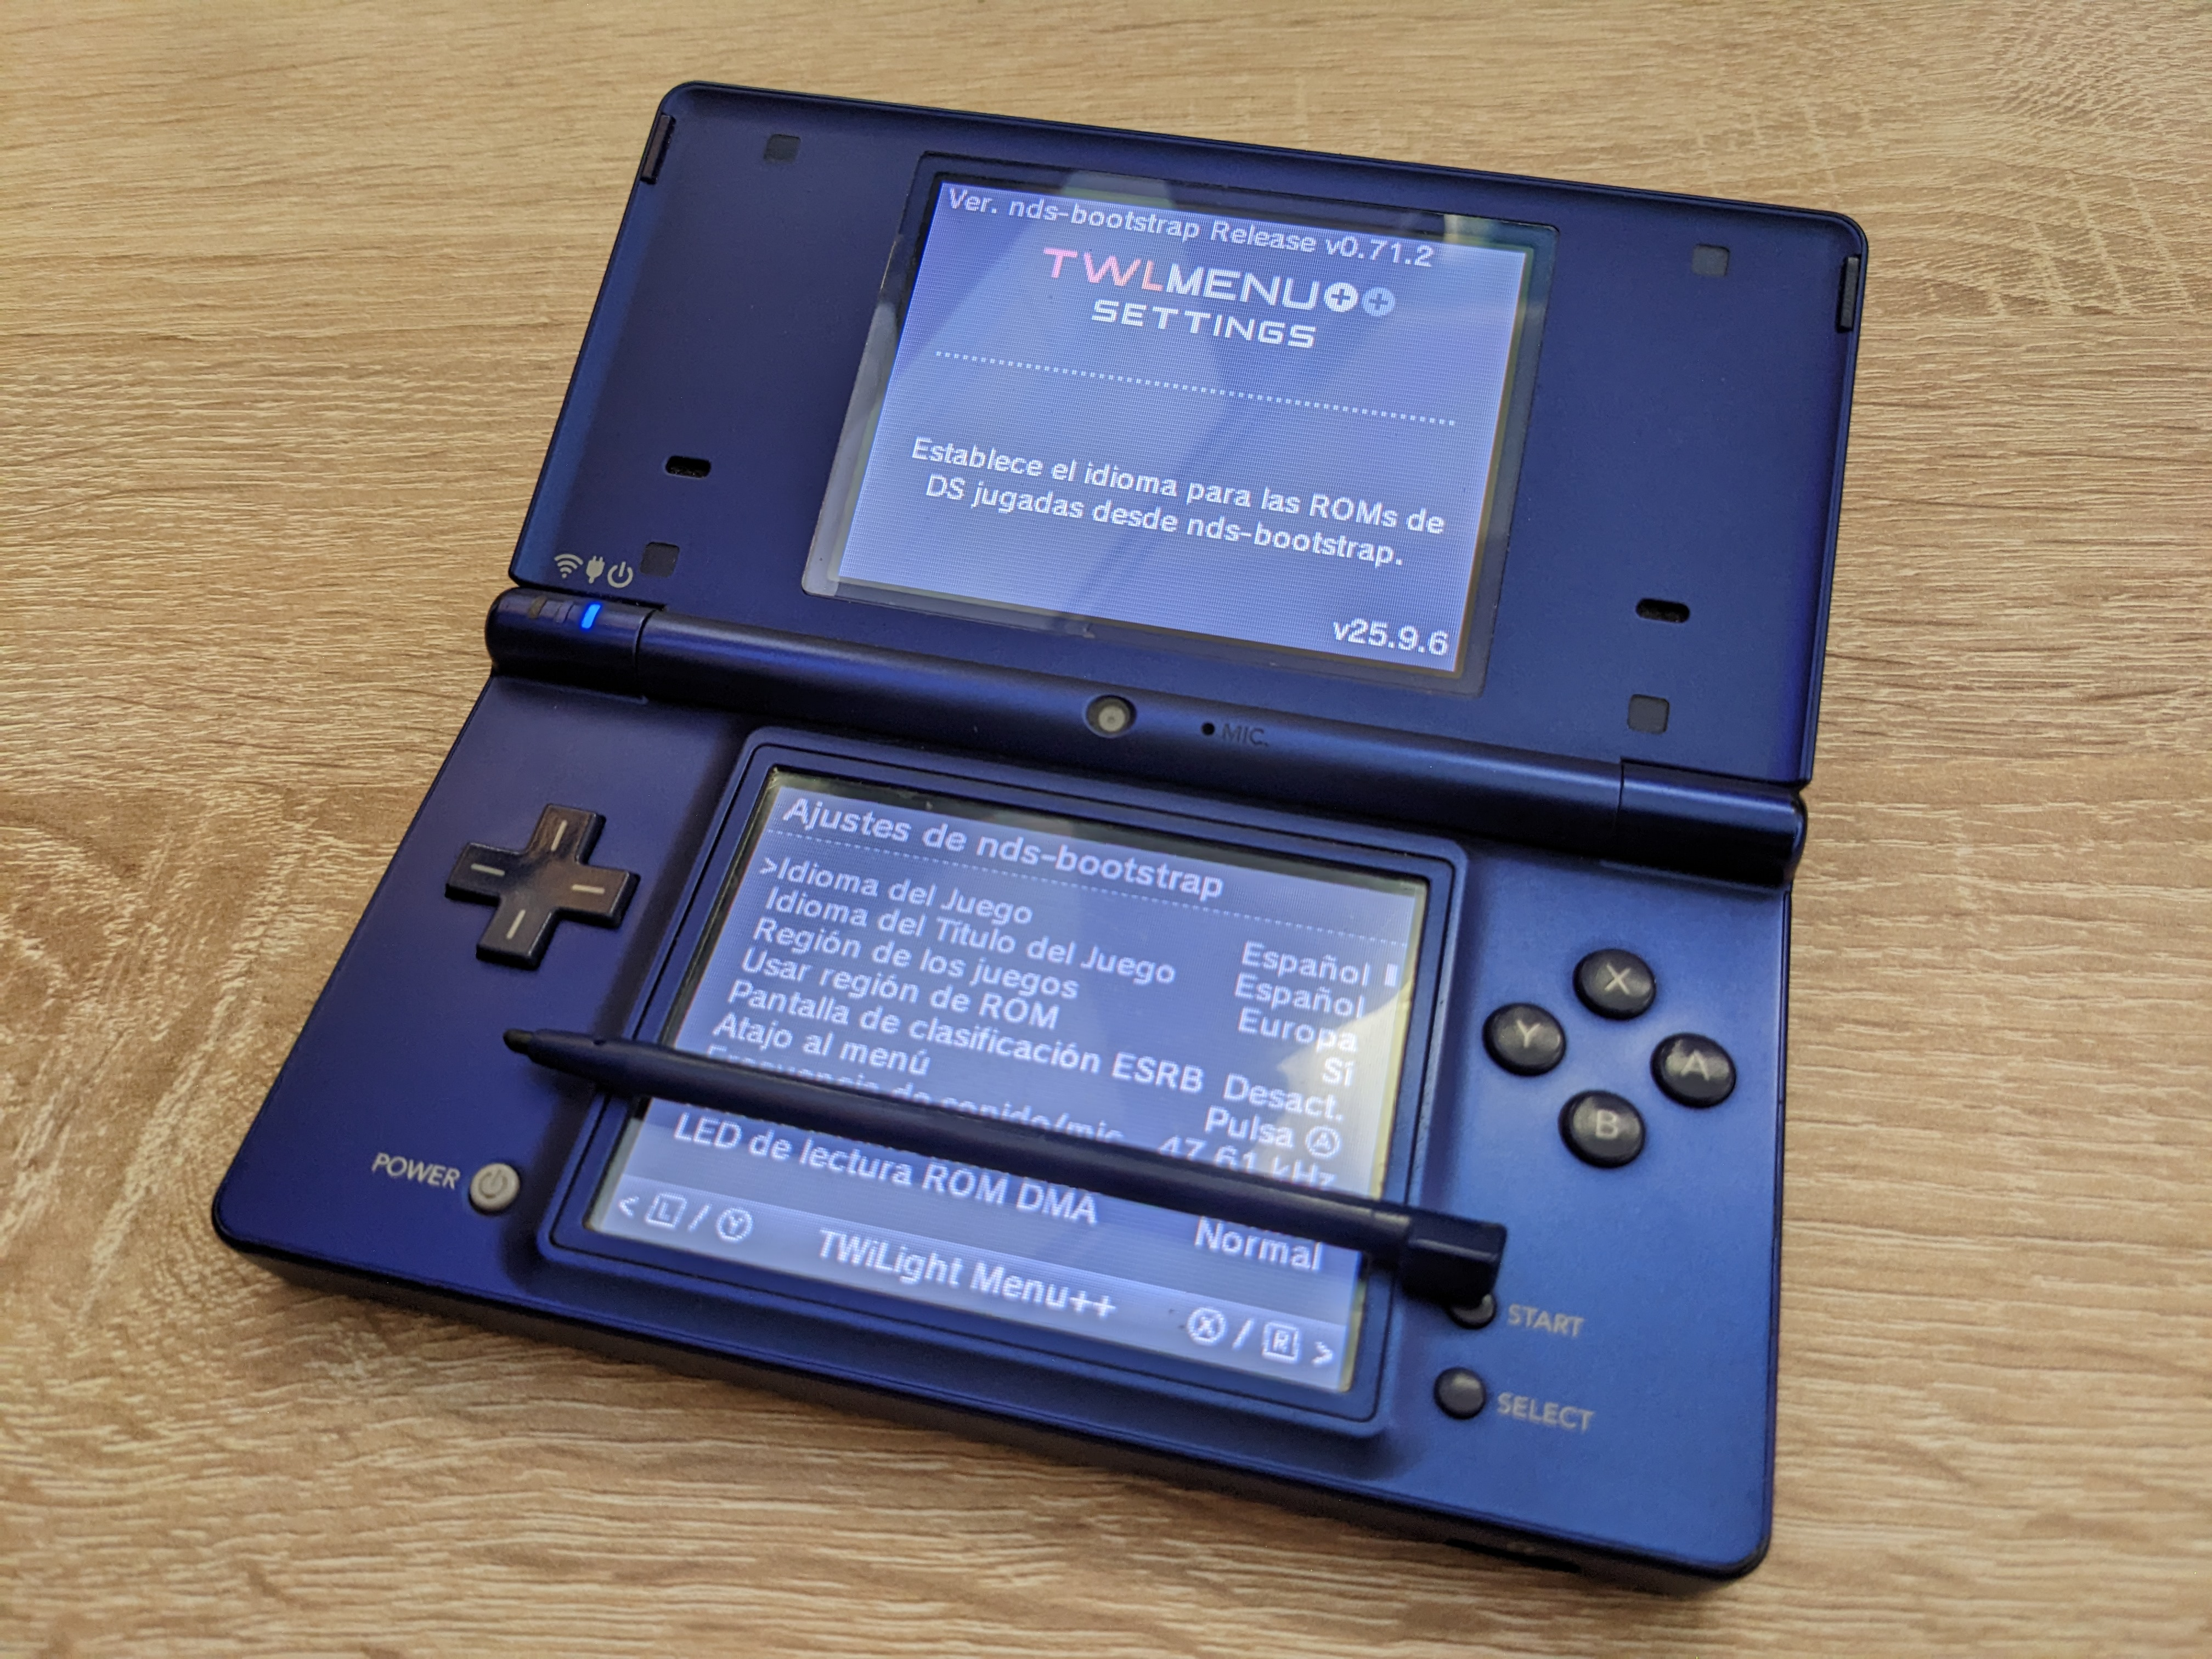
\includegraphics[width=\textwidth]{dsi.jpg}
            \caption*{\footnotesize{\textit{Nintendo DSi con Homebrew y emulador de NDS}}}
            \label{fig:dsi}
        \end{figure}

        {\large
        Jesús Jiménez Montero \\
        \par}
        \vspace{1cm}
        \hrule
        \vspace{1cm}

        {\large
        \textit{Versión 4: ALU\\
        Fecha: 09/10/2023}
        \par}
        \end{center}
\end{titlepage}

% ÍNDICE
%\renewcommand{\tableofcontents}{Indice general}
\newpage
\renewcommand{\contentsname}{Tabla de contenidos}
\setcounter{secnumdepth}{5}
\tableofcontents
\setcounter{tocdepth}{4}

\newpage
%-----------------------------------------------------------------
%-----------------------------------------------------------------
% Tabla de figuras
\newpage
\renewcommand{\listfigurename}{Lista de figuras}
\thispagestyle{empty}
\listoffigures
\newpage

\renewcommand{\listtablename}{Lista de tablas}
\listoftables
\newpage

%-----------------------------------------------------------------
%-----------------------------------------------------------------

%%%%%%%%%%%%%%%%%%%%%%%%%%%%%%%%%%%%%%%%%%%%%%%%%%%%%%%%%%%%%%%%%%%%%%%%%%
%%%%%%%%%%%%%%%%%%%%%%%%%%%%%%%%%%%%%%%%%%%%%%%%%%%%%%%%%%%%%%%%%%%%%%%%%%
\section{Registro de 1bit}
	\subsection{Tabla de verdad y explicación del circuito}

	\subsection{Esquema del circuito exterior y exterior}
		\begin{figure}[H]
			\centering
			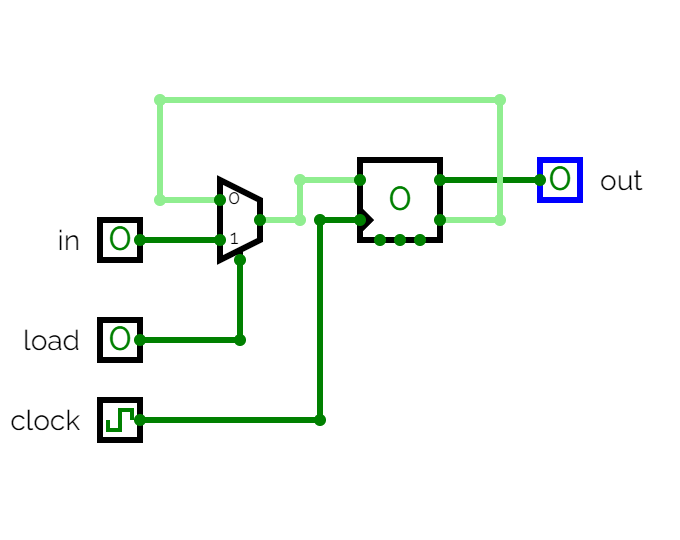
\includegraphics[width=0.75\linewidth]{RAM/REG1Bit.png}
			\caption{Esquema interior de un registro de 1 bit.}
			\label{fig:reg1bit}
		\end{figure}
	\subsection{Implementación HDL}

		\subsubsection{Archivo .HDL}
			\begin{lstlisting}

			\end{lstlisting}
		\subsubsection{Archivo .TST}
			\begin{lstlisting}

			\end{lstlisting}
		\subsubsection{Archivo .CMP}
			\begin{lstlisting}

			\end{lstlisting}
\newpage
%%%%%%%%%%%%%%%%%%%%%%%%%%%%%%%%%%%%%%%%%%%%%%%%%%%%%%%%%%%%%%%%%%%%%%%%%%
%%%%%%%%%%%%%%%%%%%%%%%%%%%%%%%%%%%%%%%%%%%%%%%%%%%%%%%%%%%%%%%%%%%%%%%%%%

\printbibliography[heading=bibintoc]
\end{document}
